\documentclass[a4paper]{book}
\usepackage{a4wide}
\usepackage{makeidx}
\usepackage{graphicx}
\usepackage{multicol}
\usepackage{float}
\usepackage{listings}
\usepackage{color}
\usepackage{textcomp}
\usepackage{alltt}
\usepackage{times}
\usepackage{ifpdf}
\ifpdf
\usepackage[pdftex,
            pagebackref=true,
            colorlinks=true,
            linkcolor=blue,
            unicode
           ]{hyperref}
\else
\usepackage[ps2pdf,
            pagebackref=true,
            colorlinks=true,
            linkcolor=blue,
            unicode
           ]{hyperref}
\usepackage{pspicture}
\fi
\usepackage[utf8]{inputenc}
\usepackage{doxygen}
\lstset{language=C++,inputencoding=utf8,basicstyle=\footnotesize,breaklines=true,breakatwhitespace=true,tabsize=8,numbers=left }
\makeindex
\setcounter{tocdepth}{3}
\renewcommand{\footrulewidth}{0.4pt}
\begin{document}
\hypersetup{pageanchor=false}
\begin{titlepage}
\vspace*{7cm}
\begin{center}
{\Large Reference Manual}\\
\vspace*{1cm}
{\large Generated by Doxygen 1.7.1}\\
\vspace*{0.5cm}
{\small Thu Jul 12 2012 17:37:22}\\
\end{center}
\end{titlepage}
\clearemptydoublepage
\pagenumbering{roman}
\tableofcontents
\clearemptydoublepage
\pagenumbering{arabic}
\hypersetup{pageanchor=true}
\chapter{Class Index}
\section{Class Hierarchy}
This inheritance list is sorted roughly, but not completely, alphabetically:\begin{DoxyCompactList}
\item \contentsline{section}{python::streamserver::server::liveStreamServer::LiveProtocol}{\pageref{classpython_1_1streamserver_1_1server_1_1liveStreamServer_1_1LiveProtocol}}{}
\item \contentsline{section}{python::streamserver::server::liveStreamServer::LiveServer}{\pageref{classpython_1_1streamserver_1_1server_1_1liveStreamServer_1_1LiveServer}}{}
\item \contentsline{section}{python::streamserver::server::source::LiveSource}{\pageref{classpython_1_1streamserver_1_1server_1_1source_1_1LiveSource}}{}
\item \contentsline{section}{python::streamserver::server::parser::NaluParser}{\pageref{classpython_1_1streamserver_1_1server_1_1parser_1_1NaluParser}}{}
\item \contentsline{section}{python::streamserver::server::source::NoSDPState}{\pageref{classpython_1_1streamserver_1_1server_1_1source_1_1NoSDPState}}{}
\item \contentsline{section}{python::streamserver::server::rtspHandler::RTSPRequestHandler}{\pageref{classpython_1_1streamserver_1_1server_1_1rtspHandler_1_1RTSPRequestHandler}}{}
\item \contentsline{section}{python::streamserver::server::rtspServer::RTSPServerFactory}{\pageref{classpython_1_1streamserver_1_1server_1_1rtspServer_1_1RTSPServerFactory}}{}
\item \contentsline{section}{python::streamserver::server::rtspServer::RTSPServerProtocol}{\pageref{classpython_1_1streamserver_1_1server_1_1rtspServer_1_1RTSPServerProtocol}}{}
\item \contentsline{section}{python::streamserver::server::rtspServer::RTSPState}{\pageref{classpython_1_1streamserver_1_1server_1_1rtspServer_1_1RTSPState}}{}
\begin{DoxyCompactList}
\item \contentsline{section}{python::streamserver::server::rtspServer::RTSPInitState}{\pageref{classpython_1_1streamserver_1_1server_1_1rtspServer_1_1RTSPInitState}}{}
\item \contentsline{section}{python::streamserver::server::rtspServer::RTSPPlayingState}{\pageref{classpython_1_1streamserver_1_1server_1_1rtspServer_1_1RTSPPlayingState}}{}
\item \contentsline{section}{python::streamserver::server::rtspServer::RTSPReadyState}{\pageref{classpython_1_1streamserver_1_1server_1_1rtspServer_1_1RTSPReadyState}}{}
\end{DoxyCompactList}
\item \contentsline{section}{python::streamserver::server::source::SDPState}{\pageref{classpython_1_1streamserver_1_1server_1_1source_1_1SDPState}}{}
\end{DoxyCompactList}

\chapter{Class Index}
\section{Class List}
Here are the classes, structs, unions and interfaces with brief descriptions:\begin{DoxyCompactList}
\item\contentsline{section}{\hyperlink{classpython_1_1streamserver_1_1server_1_1liveStreamServer_1_1LiveProtocol}{python::streamserver::server::liveStreamServer::LiveProtocol} }{\pageref{classpython_1_1streamserver_1_1server_1_1liveStreamServer_1_1LiveProtocol}}{}
\item\contentsline{section}{\hyperlink{classpython_1_1streamserver_1_1server_1_1liveStreamServer_1_1LiveServer}{python::streamserver::server::liveStreamServer::LiveServer} }{\pageref{classpython_1_1streamserver_1_1server_1_1liveStreamServer_1_1LiveServer}}{}
\item\contentsline{section}{\hyperlink{classpython_1_1streamserver_1_1server_1_1source_1_1LiveSource}{python::streamserver::server::source::LiveSource} }{\pageref{classpython_1_1streamserver_1_1server_1_1source_1_1LiveSource}}{}
\item\contentsline{section}{\hyperlink{classpython_1_1streamserver_1_1server_1_1parser_1_1NaluParser}{python::streamserver::server::parser::NaluParser} }{\pageref{classpython_1_1streamserver_1_1server_1_1parser_1_1NaluParser}}{}
\item\contentsline{section}{\hyperlink{classpython_1_1streamserver_1_1server_1_1source_1_1NoSDPState}{python::streamserver::server::source::NoSDPState} }{\pageref{classpython_1_1streamserver_1_1server_1_1source_1_1NoSDPState}}{}
\item\contentsline{section}{\hyperlink{classpython_1_1streamserver_1_1server_1_1rtspServer_1_1RTSPInitState}{python::streamserver::server::rtspServer::RTSPInitState} }{\pageref{classpython_1_1streamserver_1_1server_1_1rtspServer_1_1RTSPInitState}}{}
\item\contentsline{section}{\hyperlink{classpython_1_1streamserver_1_1server_1_1rtspServer_1_1RTSPPlayingState}{python::streamserver::server::rtspServer::RTSPPlayingState} }{\pageref{classpython_1_1streamserver_1_1server_1_1rtspServer_1_1RTSPPlayingState}}{}
\item\contentsline{section}{\hyperlink{classpython_1_1streamserver_1_1server_1_1rtspServer_1_1RTSPReadyState}{python::streamserver::server::rtspServer::RTSPReadyState} }{\pageref{classpython_1_1streamserver_1_1server_1_1rtspServer_1_1RTSPReadyState}}{}
\item\contentsline{section}{\hyperlink{classpython_1_1streamserver_1_1server_1_1rtspHandler_1_1RTSPRequestHandler}{python::streamserver::server::rtspHandler::RTSPRequestHandler} }{\pageref{classpython_1_1streamserver_1_1server_1_1rtspHandler_1_1RTSPRequestHandler}}{}
\item\contentsline{section}{\hyperlink{classpython_1_1streamserver_1_1server_1_1rtspServer_1_1RTSPServerFactory}{python::streamserver::server::rtspServer::RTSPServerFactory} }{\pageref{classpython_1_1streamserver_1_1server_1_1rtspServer_1_1RTSPServerFactory}}{}
\item\contentsline{section}{\hyperlink{classpython_1_1streamserver_1_1server_1_1rtspServer_1_1RTSPServerProtocol}{python::streamserver::server::rtspServer::RTSPServerProtocol} }{\pageref{classpython_1_1streamserver_1_1server_1_1rtspServer_1_1RTSPServerProtocol}}{}
\item\contentsline{section}{\hyperlink{classpython_1_1streamserver_1_1server_1_1rtspServer_1_1RTSPState}{python::streamserver::server::rtspServer::RTSPState} }{\pageref{classpython_1_1streamserver_1_1server_1_1rtspServer_1_1RTSPState}}{}
\item\contentsline{section}{\hyperlink{classpython_1_1streamserver_1_1server_1_1source_1_1SDPState}{python::streamserver::server::source::SDPState} }{\pageref{classpython_1_1streamserver_1_1server_1_1source_1_1SDPState}}{}
\end{DoxyCompactList}

\chapter{File Index}
\section{File List}
Here is a list of all documented files with brief descriptions:\begin{DoxyCompactList}
\item\contentsline{section}{/home/yy/programme/python/streamserver/server/\hyperlink{liveStreamServer_8py}{liveStreamServer.py} (Accpept live stream )}{\pageref{liveStreamServer_8py}}{}
\item\contentsline{section}{/home/yy/programme/python/streamserver/server/\hyperlink{parser_8py}{parser.py} (Extract the SDP and each frame from the nalu )}{\pageref{parser_8py}}{}
\item\contentsline{section}{/home/yy/programme/python/streamserver/server/\hyperlink{rtspHandler_8py}{rtspHandler.py} (Details of handle rtsp request )}{\pageref{rtspHandler_8py}}{}
\item\contentsline{section}{/home/yy/programme/python/streamserver/server/\hyperlink{rtspServer_8py}{rtspServer.py} (Start rtsp session and setup connection with the player )}{\pageref{rtspServer_8py}}{}
\item\contentsline{section}{/home/yy/programme/python/streamserver/server/\hyperlink{source_8py}{source.py} (LiveSource and FileSource )}{\pageref{source_8py}}{}
\end{DoxyCompactList}

\chapter{Class Documentation}
\hypertarget{classpython_1_1streamserver_1_1server_1_1liveStreamServer_1_1LiveProtocol}{
\section{python::streamserver::server::liveStreamServer::LiveProtocol Class Reference}
\label{classpython_1_1streamserver_1_1server_1_1liveStreamServer_1_1LiveProtocol}\index{python::streamserver::server::liveStreamServer::LiveProtocol@{python::streamserver::server::liveStreamServer::LiveProtocol}}
}
\subsection*{Public Member Functions}
\begin{DoxyCompactItemize}
\item 
\hypertarget{classpython_1_1streamserver_1_1server_1_1liveStreamServer_1_1LiveProtocol_a70114a4d7d6387a741fd0b2263705044}{
def {\bfseries \_\-\_\-init\_\-\_\-}}
\label{classpython_1_1streamserver_1_1server_1_1liveStreamServer_1_1LiveProtocol_a70114a4d7d6387a741fd0b2263705044}

\item 
\hypertarget{classpython_1_1streamserver_1_1server_1_1liveStreamServer_1_1LiveProtocol_aba2235e748d6a4ebf7fedcd45e5ad24d}{
def {\bfseries getSource}}
\label{classpython_1_1streamserver_1_1server_1_1liveStreamServer_1_1LiveProtocol_aba2235e748d6a4ebf7fedcd45e5ad24d}

\item 
\hypertarget{classpython_1_1streamserver_1_1server_1_1liveStreamServer_1_1LiveProtocol_a7bbb23a4a4a84fdd17c85dbdb24d9774}{
def {\bfseries connectionMade}}
\label{classpython_1_1streamserver_1_1server_1_1liveStreamServer_1_1LiveProtocol_a7bbb23a4a4a84fdd17c85dbdb24d9774}

\item 
\hypertarget{classpython_1_1streamserver_1_1server_1_1liveStreamServer_1_1LiveProtocol_a320597763f8fda88b5bf946d2a536a3d}{
def {\bfseries lineReceived}}
\label{classpython_1_1streamserver_1_1server_1_1liveStreamServer_1_1LiveProtocol_a320597763f8fda88b5bf946d2a536a3d}

\item 
\hypertarget{classpython_1_1streamserver_1_1server_1_1liveStreamServer_1_1LiveProtocol_ab6e5d4cff0750188eca6d5a2aeff0b8f}{
def {\bfseries connectionLost}}
\label{classpython_1_1streamserver_1_1server_1_1liveStreamServer_1_1LiveProtocol_ab6e5d4cff0750188eca6d5a2aeff0b8f}

\end{DoxyCompactItemize}
\subsection*{Static Public Attributes}
\begin{DoxyCompactItemize}
\item 
\hypertarget{classpython_1_1streamserver_1_1server_1_1liveStreamServer_1_1LiveProtocol_a8f1edd568d95101888a5dc692ca83503}{
string {\bfseries delimiter} = '$\backslash$x00$\backslash$x00$\backslash$x00$\backslash$x01'}
\label{classpython_1_1streamserver_1_1server_1_1liveStreamServer_1_1LiveProtocol_a8f1edd568d95101888a5dc692ca83503}

\end{DoxyCompactItemize}


\subsection{Detailed Description}
\begin{DoxyVerb}accept live stream data and parse it\end{DoxyVerb}
 

The documentation for this class was generated from the following file:\begin{DoxyCompactItemize}
\item 
/home/yy/programme/python/streamserver/server/\hyperlink{liveStreamServer_8py}{liveStreamServer.py}\end{DoxyCompactItemize}

\hypertarget{classpython_1_1streamserver_1_1server_1_1liveStreamServer_1_1LiveServer}{
\section{python::streamserver::server::liveStreamServer::LiveServer Class Reference}
\label{classpython_1_1streamserver_1_1server_1_1liveStreamServer_1_1LiveServer}\index{python::streamserver::server::liveStreamServer::LiveServer@{python::streamserver::server::liveStreamServer::LiveServer}}
}
\subsection*{Public Member Functions}
\begin{DoxyCompactItemize}
\item 
\hypertarget{classpython_1_1streamserver_1_1server_1_1liveStreamServer_1_1LiveServer_a8ce5d7732b79eb00ff858f6a534379cd}{
def {\bfseries \_\-\_\-init\_\-\_\-}}
\label{classpython_1_1streamserver_1_1server_1_1liveStreamServer_1_1LiveServer_a8ce5d7732b79eb00ff858f6a534379cd}

\item 
\hypertarget{classpython_1_1streamserver_1_1server_1_1liveStreamServer_1_1LiveServer_a4f89db5ba67e4935ef1bee02747bf471}{
def {\bfseries getClientNum}}
\label{classpython_1_1streamserver_1_1server_1_1liveStreamServer_1_1LiveServer_a4f89db5ba67e4935ef1bee02747bf471}

\item 
\hypertarget{classpython_1_1streamserver_1_1server_1_1liveStreamServer_1_1LiveServer_a3eb0b689e1f37e02767f331f6b7adf2a}{
def {\bfseries buildProtocol}}
\label{classpython_1_1streamserver_1_1server_1_1liveStreamServer_1_1LiveServer_a3eb0b689e1f37e02767f331f6b7adf2a}

\item 
\hypertarget{classpython_1_1streamserver_1_1server_1_1liveStreamServer_1_1LiveServer_a5d19a7865163749a162f98f79442f7fc}{
def {\bfseries connectionLost}}
\label{classpython_1_1streamserver_1_1server_1_1liveStreamServer_1_1LiveServer_a5d19a7865163749a162f98f79442f7fc}

\end{DoxyCompactItemize}
\subsection*{Static Public Attributes}
\begin{DoxyCompactItemize}
\item 
\hypertarget{classpython_1_1streamserver_1_1server_1_1liveStreamServer_1_1LiveServer_a48cef0fd3f41dc26c8020667cffffe33}{
{\bfseries protocol} = \hyperlink{classpython_1_1streamserver_1_1server_1_1liveStreamServer_1_1LiveProtocol}{LiveProtocol}}
\label{classpython_1_1streamserver_1_1server_1_1liveStreamServer_1_1LiveServer_a48cef0fd3f41dc26c8020667cffffe33}

\end{DoxyCompactItemize}


\subsection{Detailed Description}
\begin{DoxyVerb}listen for live stream connection\end{DoxyVerb}
 

The documentation for this class was generated from the following file:\begin{DoxyCompactItemize}
\item 
/home/yy/programme/python/streamserver/server/\hyperlink{liveStreamServer_8py}{liveStreamServer.py}\end{DoxyCompactItemize}

\hypertarget{classpython_1_1streamserver_1_1server_1_1source_1_1LiveSource}{
\section{python::streamserver::server::source::LiveSource Class Reference}
\label{classpython_1_1streamserver_1_1server_1_1source_1_1LiveSource}\index{python::streamserver::server::source::LiveSource@{python::streamserver::server::source::LiveSource}}
}
\subsection*{Public Member Functions}
\begin{DoxyCompactItemize}
\item 
\hypertarget{classpython_1_1streamserver_1_1server_1_1source_1_1LiveSource_a3113b53aec3915a8a76a985843a39471}{
def {\bfseries \_\-\_\-init\_\-\_\-}}
\label{classpython_1_1streamserver_1_1server_1_1source_1_1LiveSource_a3113b53aec3915a8a76a985843a39471}

\item 
\hypertarget{classpython_1_1streamserver_1_1server_1_1source_1_1LiveSource_abe5c08b4ebb2ae07b7affbc054d31d7f}{
def {\bfseries getName}}
\label{classpython_1_1streamserver_1_1server_1_1source_1_1LiveSource_abe5c08b4ebb2ae07b7affbc054d31d7f}

\item 
\hypertarget{classpython_1_1streamserver_1_1server_1_1source_1_1LiveSource_aa8bcdf70f7f25a5192c49a43aef92095}{
def {\bfseries getSDP}}
\label{classpython_1_1streamserver_1_1server_1_1source_1_1LiveSource_aa8bcdf70f7f25a5192c49a43aef92095}

\item 
\hypertarget{classpython_1_1streamserver_1_1server_1_1source_1_1LiveSource_abc14e1ea625fde206b1e318991a68ee8}{
def {\bfseries setSDP}}
\label{classpython_1_1streamserver_1_1server_1_1source_1_1LiveSource_abc14e1ea625fde206b1e318991a68ee8}

\item 
\hypertarget{classpython_1_1streamserver_1_1server_1_1source_1_1LiveSource_ac4bf895acd0df37b088001cfb524b736}{
def {\bfseries setState}}
\label{classpython_1_1streamserver_1_1server_1_1source_1_1LiveSource_ac4bf895acd0df37b088001cfb524b736}

\item 
\hypertarget{classpython_1_1streamserver_1_1server_1_1source_1_1LiveSource_af9925d56c5c11dc853e144a5d5a12806}{
def {\bfseries getState}}
\label{classpython_1_1streamserver_1_1server_1_1source_1_1LiveSource_af9925d56c5c11dc853e144a5d5a12806}

\item 
def \hyperlink{classpython_1_1streamserver_1_1server_1_1source_1_1LiveSource_ad47941d73793e83d4a12e669c2d166b0}{pauseProducing}
\item 
\hypertarget{classpython_1_1streamserver_1_1server_1_1source_1_1LiveSource_a80e3fd39e5fd0027e69849a4afdc8905}{
def {\bfseries resumeProducing}}
\label{classpython_1_1streamserver_1_1server_1_1source_1_1LiveSource_a80e3fd39e5fd0027e69849a4afdc8905}

\item 
\hypertarget{classpython_1_1streamserver_1_1server_1_1source_1_1LiveSource_a9cc460c4ed10aefa69409f6e29020936}{
def {\bfseries stopProducing}}
\label{classpython_1_1streamserver_1_1server_1_1source_1_1LiveSource_a9cc460c4ed10aefa69409f6e29020936}

\item 
\hypertarget{classpython_1_1streamserver_1_1server_1_1source_1_1LiveSource_a4581b650fcb2d690571909ee5625e30d}{
def {\bfseries parseNalu}}
\label{classpython_1_1streamserver_1_1server_1_1source_1_1LiveSource_a4581b650fcb2d690571909ee5625e30d}

\end{DoxyCompactItemize}
\subsection*{Static Public Attributes}
\begin{DoxyCompactItemize}
\item 
\hypertarget{classpython_1_1streamserver_1_1server_1_1source_1_1LiveSource_a548a3c84d07ade1b6e147b3376ff75c2}{
tuple {\bfseries noSDPState} = \hyperlink{classpython_1_1streamserver_1_1server_1_1source_1_1NoSDPState}{NoSDPState}()}
\label{classpython_1_1streamserver_1_1server_1_1source_1_1LiveSource_a548a3c84d07ade1b6e147b3376ff75c2}

\item 
\hypertarget{classpython_1_1streamserver_1_1server_1_1source_1_1LiveSource_aa77a75961ae9e8fbfa7a6aa3cc4dd775}{
tuple {\bfseries hasSDPState} = \hyperlink{classpython_1_1streamserver_1_1server_1_1source_1_1SDPState}{SDPState}()}
\label{classpython_1_1streamserver_1_1server_1_1source_1_1LiveSource_aa77a75961ae9e8fbfa7a6aa3cc4dd775}

\end{DoxyCompactItemize}


\subsection{Detailed Description}
\begin{DoxyVerb}generate live stream source\end{DoxyVerb}
 

\subsection{Member Function Documentation}
\hypertarget{classpython_1_1streamserver_1_1server_1_1source_1_1LiveSource_ad47941d73793e83d4a12e669c2d166b0}{
\index{python::streamserver::server::source::LiveSource@{python::streamserver::server::source::LiveSource}!pauseProducing@{pauseProducing}}
\index{pauseProducing@{pauseProducing}!python::streamserver::server::source::LiveSource@{python::streamserver::server::source::LiveSource}}
\subsubsection[{pauseProducing}]{\setlength{\rightskip}{0pt plus 5cm}def python::streamserver::server::source::LiveSource::pauseProducing (
\begin{DoxyParamCaption}
\item[{}]{ self}
\end{DoxyParamCaption}
)}}
\label{classpython_1_1streamserver_1_1server_1_1source_1_1LiveSource_ad47941d73793e83d4a12e669c2d166b0}
\begin{DoxyVerb}When we've produce data too fast, pauseProducing will be called\end{DoxyVerb}
 

The documentation for this class was generated from the following file:\begin{DoxyCompactItemize}
\item 
/home/yy/programme/python/streamserver/server/\hyperlink{source_8py}{source.py}\end{DoxyCompactItemize}

\hypertarget{classpython_1_1streamserver_1_1server_1_1parser_1_1NaluParser}{
\section{python::streamserver::server::parser::NaluParser Class Reference}
\label{classpython_1_1streamserver_1_1server_1_1parser_1_1NaluParser}\index{python::streamserver::server::parser::NaluParser@{python::streamserver::server::parser::NaluParser}}
}
\subsection*{Public Member Functions}
\begin{DoxyCompactItemize}
\item 
\hypertarget{classpython_1_1streamserver_1_1server_1_1parser_1_1NaluParser_acfcfa97418b967c40e4841fd27ab607a}{
def {\bfseries generateSDP}}
\label{classpython_1_1streamserver_1_1server_1_1parser_1_1NaluParser_acfcfa97418b967c40e4841fd27ab607a}

\end{DoxyCompactItemize}


\subsection{Detailed Description}
\begin{DoxyVerb}generate SDP and extract each frame\end{DoxyVerb}
 

The documentation for this class was generated from the following file:\begin{DoxyCompactItemize}
\item 
/home/yy/programme/python/streamserver/server/\hyperlink{parser_8py}{parser.py}\end{DoxyCompactItemize}

\hypertarget{classpython_1_1streamserver_1_1server_1_1source_1_1NoSDPState}{
\section{python::streamserver::server::source::NoSDPState Class Reference}
\label{classpython_1_1streamserver_1_1server_1_1source_1_1NoSDPState}\index{python::streamserver::server::source::NoSDPState@{python::streamserver::server::source::NoSDPState}}
}
\subsection*{Public Member Functions}
\begin{DoxyCompactItemize}
\item 
\hypertarget{classpython_1_1streamserver_1_1server_1_1source_1_1NoSDPState_aa7b1020ce67ee1bca1616672cf9261d3}{
def {\bfseries \_\-\_\-init\_\-\_\-}}
\label{classpython_1_1streamserver_1_1server_1_1source_1_1NoSDPState_aa7b1020ce67ee1bca1616672cf9261d3}

\item 
\hypertarget{classpython_1_1streamserver_1_1server_1_1source_1_1NoSDPState_a312ccd7f23c70a069bdcf0232ff37d2a}{
def {\bfseries parseNalu}}
\label{classpython_1_1streamserver_1_1server_1_1source_1_1NoSDPState_a312ccd7f23c70a069bdcf0232ff37d2a}

\end{DoxyCompactItemize}


\subsection{Detailed Description}
\begin{DoxyVerb}when source hasn't generate SDP yet\end{DoxyVerb}
 

The documentation for this class was generated from the following file:\begin{DoxyCompactItemize}
\item 
/home/yy/programme/python/streamserver/server/\hyperlink{source_8py}{source.py}\end{DoxyCompactItemize}

\hypertarget{classpython_1_1streamserver_1_1server_1_1rtspServer_1_1RTSPInitState}{
\section{python::streamserver::server::rtspServer::RTSPInitState Class Reference}
\label{classpython_1_1streamserver_1_1server_1_1rtspServer_1_1RTSPInitState}\index{python::streamserver::server::rtspServer::RTSPInitState@{python::streamserver::server::rtspServer::RTSPInitState}}
}
Inheritance diagram for python::streamserver::server::rtspServer::RTSPInitState:\begin{figure}[H]
\begin{center}
\leavevmode
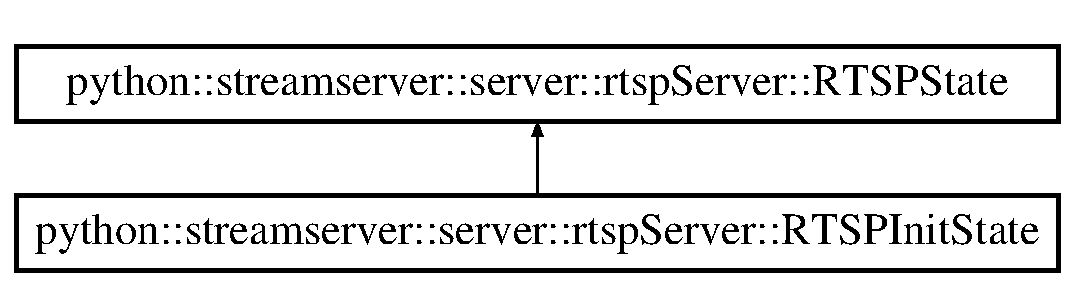
\includegraphics[height=2.000000cm]{classpython_1_1streamserver_1_1server_1_1rtspServer_1_1RTSPInitState}
\end{center}
\end{figure}
\subsection*{Public Member Functions}
\begin{DoxyCompactItemize}
\item 
\hypertarget{classpython_1_1streamserver_1_1server_1_1rtspServer_1_1RTSPInitState_ae3bae13f081bcffe0826f0ff3a1ef3bd}{
def {\bfseries handleSETUP}}
\label{classpython_1_1streamserver_1_1server_1_1rtspServer_1_1RTSPInitState_ae3bae13f081bcffe0826f0ff3a1ef3bd}

\item 
\hypertarget{classpython_1_1streamserver_1_1server_1_1rtspServer_1_1RTSPInitState_acddd622ba247fcbf69e81a15b7e47199}{
def {\bfseries handlePLAY}}
\label{classpython_1_1streamserver_1_1server_1_1rtspServer_1_1RTSPInitState_acddd622ba247fcbf69e81a15b7e47199}

\item 
\hypertarget{classpython_1_1streamserver_1_1server_1_1rtspServer_1_1RTSPInitState_aef7d512356f85d4b1e0aa9d603d1ede8}{
def {\bfseries handleTEARDOWN}}
\label{classpython_1_1streamserver_1_1server_1_1rtspServer_1_1RTSPInitState_aef7d512356f85d4b1e0aa9d603d1ede8}

\end{DoxyCompactItemize}


\subsection{Detailed Description}
\begin{DoxyVerb}message received    next state
        SETUP               Ready
        TEARDOWN            Init\end{DoxyVerb}
 

The documentation for this class was generated from the following file:\begin{DoxyCompactItemize}
\item 
/home/yy/programme/python/streamserver/server/\hyperlink{rtspServer_8py}{rtspServer.py}\end{DoxyCompactItemize}

\hypertarget{classpython_1_1streamserver_1_1server_1_1rtspServer_1_1RTSPPlayingState}{
\section{python::streamserver::server::rtspServer::RTSPPlayingState Class Reference}
\label{classpython_1_1streamserver_1_1server_1_1rtspServer_1_1RTSPPlayingState}\index{python::streamserver::server::rtspServer::RTSPPlayingState@{python::streamserver::server::rtspServer::RTSPPlayingState}}
}
Inheritance diagram for python::streamserver::server::rtspServer::RTSPPlayingState:\begin{figure}[H]
\begin{center}
\leavevmode
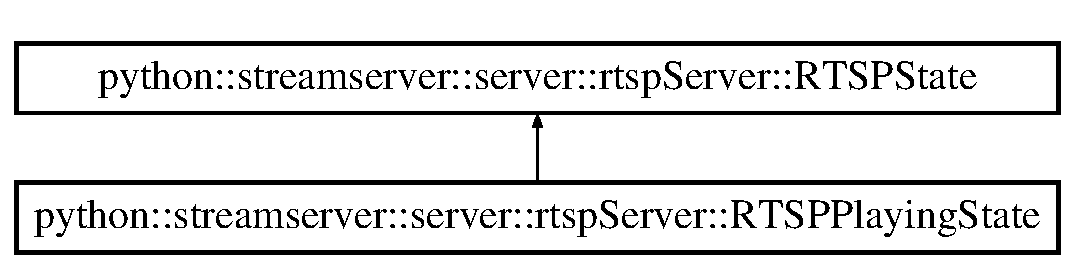
\includegraphics[height=2.000000cm]{classpython_1_1streamserver_1_1server_1_1rtspServer_1_1RTSPPlayingState}
\end{center}
\end{figure}
\subsection*{Public Member Functions}
\begin{DoxyCompactItemize}
\item 
\hypertarget{classpython_1_1streamserver_1_1server_1_1rtspServer_1_1RTSPPlayingState_a5597a91d11df6aeaf316020db662842f}{
def {\bfseries handleSETUP}}
\label{classpython_1_1streamserver_1_1server_1_1rtspServer_1_1RTSPPlayingState_a5597a91d11df6aeaf316020db662842f}

\item 
\hypertarget{classpython_1_1streamserver_1_1server_1_1rtspServer_1_1RTSPPlayingState_a9abc670a45c75206620433616d8b3ca2}{
def {\bfseries handlePLAY}}
\label{classpython_1_1streamserver_1_1server_1_1rtspServer_1_1RTSPPlayingState_a9abc670a45c75206620433616d8b3ca2}

\item 
\hypertarget{classpython_1_1streamserver_1_1server_1_1rtspServer_1_1RTSPPlayingState_a16dcc5de6225033e57f9445f13cd872c}{
def {\bfseries handleTEARDOWN}}
\label{classpython_1_1streamserver_1_1server_1_1rtspServer_1_1RTSPPlayingState_a16dcc5de6225033e57f9445f13cd872c}

\end{DoxyCompactItemize}


\subsection{Detailed Description}
\begin{DoxyVerb}message received    next state
        SETUP               Playing 
        TEARDOWN            Init
        PLAY                Playing\end{DoxyVerb}
 

The documentation for this class was generated from the following file:\begin{DoxyCompactItemize}
\item 
/home/yy/programme/python/streamserver/server/\hyperlink{rtspServer_8py}{rtspServer.py}\end{DoxyCompactItemize}

\hypertarget{classpython_1_1streamserver_1_1server_1_1rtspServer_1_1RTSPReadyState}{
\section{python::streamserver::server::rtspServer::RTSPReadyState Class Reference}
\label{classpython_1_1streamserver_1_1server_1_1rtspServer_1_1RTSPReadyState}\index{python::streamserver::server::rtspServer::RTSPReadyState@{python::streamserver::server::rtspServer::RTSPReadyState}}
}
Inheritance diagram for python::streamserver::server::rtspServer::RTSPReadyState:\begin{figure}[H]
\begin{center}
\leavevmode
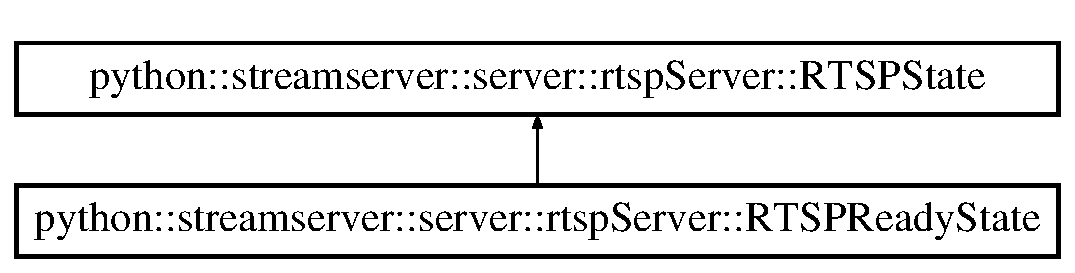
\includegraphics[height=2.000000cm]{classpython_1_1streamserver_1_1server_1_1rtspServer_1_1RTSPReadyState}
\end{center}
\end{figure}
\subsection*{Public Member Functions}
\begin{DoxyCompactItemize}
\item 
\hypertarget{classpython_1_1streamserver_1_1server_1_1rtspServer_1_1RTSPReadyState_a81962d804179d9b796b820644a27b5c8}{
def {\bfseries handleSETUP}}
\label{classpython_1_1streamserver_1_1server_1_1rtspServer_1_1RTSPReadyState_a81962d804179d9b796b820644a27b5c8}

\item 
\hypertarget{classpython_1_1streamserver_1_1server_1_1rtspServer_1_1RTSPReadyState_ad013997941e8969f410b550318c683c8}{
def {\bfseries handlePLAY}}
\label{classpython_1_1streamserver_1_1server_1_1rtspServer_1_1RTSPReadyState_ad013997941e8969f410b550318c683c8}

\item 
\hypertarget{classpython_1_1streamserver_1_1server_1_1rtspServer_1_1RTSPReadyState_a1a1c6914b0b6d949b7f55cfdd636fccc}{
def {\bfseries handleTEARDOWN}}
\label{classpython_1_1streamserver_1_1server_1_1rtspServer_1_1RTSPReadyState_a1a1c6914b0b6d949b7f55cfdd636fccc}

\end{DoxyCompactItemize}


\subsection{Detailed Description}
\begin{DoxyVerb}message received    next state
        SETUP               Ready
        TEARDOWN            Init
        PLAY                Playing\end{DoxyVerb}
 

The documentation for this class was generated from the following file:\begin{DoxyCompactItemize}
\item 
/home/yy/programme/python/streamserver/server/\hyperlink{rtspServer_8py}{rtspServer.py}\end{DoxyCompactItemize}

\hypertarget{classpython_1_1streamserver_1_1server_1_1rtspHandler_1_1RTSPRequestHandler}{
\section{python::streamserver::server::rtspHandler::RTSPRequestHandler Class Reference}
\label{classpython_1_1streamserver_1_1server_1_1rtspHandler_1_1RTSPRequestHandler}\index{python::streamserver::server::rtspHandler::RTSPRequestHandler@{python::streamserver::server::rtspHandler::RTSPRequestHandler}}
}
\subsection*{Public Member Functions}
\begin{DoxyCompactItemize}
\item 
\hypertarget{classpython_1_1streamserver_1_1server_1_1rtspHandler_1_1RTSPRequestHandler_a32a8f95264daf589e178bdf421d681e9}{
def {\bfseries \_\-\_\-init\_\-\_\-}}
\label{classpython_1_1streamserver_1_1server_1_1rtspHandler_1_1RTSPRequestHandler_a32a8f95264daf589e178bdf421d681e9}

\item 
\hypertarget{classpython_1_1streamserver_1_1server_1_1rtspHandler_1_1RTSPRequestHandler_aaa78bcfabbe0df852f1f6ad0003de2c6}{
def {\bfseries parseCSeq}}
\label{classpython_1_1streamserver_1_1server_1_1rtspHandler_1_1RTSPRequestHandler_aaa78bcfabbe0df852f1f6ad0003de2c6}

\item 
\hypertarget{classpython_1_1streamserver_1_1server_1_1rtspHandler_1_1RTSPRequestHandler_adc3c9ce4aea84c327ac493cb8a0ee2b0}{
def {\bfseries handleOPTIONS}}
\label{classpython_1_1streamserver_1_1server_1_1rtspHandler_1_1RTSPRequestHandler_adc3c9ce4aea84c327ac493cb8a0ee2b0}

\item 
\hypertarget{classpython_1_1streamserver_1_1server_1_1rtspHandler_1_1RTSPRequestHandler_a5eb6ba4ed5ec8c8c80d192ae0808c1b6}{
def {\bfseries handleDESCRIBE}}
\label{classpython_1_1streamserver_1_1server_1_1rtspHandler_1_1RTSPRequestHandler_a5eb6ba4ed5ec8c8c80d192ae0808c1b6}

\item 
\hypertarget{classpython_1_1streamserver_1_1server_1_1rtspHandler_1_1RTSPRequestHandler_a487523a7e2efa0b81f9415ddf0dba843}{
def {\bfseries findSource}}
\label{classpython_1_1streamserver_1_1server_1_1rtspHandler_1_1RTSPRequestHandler_a487523a7e2efa0b81f9415ddf0dba843}

\end{DoxyCompactItemize}
\subsection*{Public Attributes}
\begin{DoxyCompactItemize}
\item 
\hypertarget{classpython_1_1streamserver_1_1server_1_1rtspHandler_1_1RTSPRequestHandler_aebbdf12429f04728ce841d8f7fa462d3}{
{\bfseries sessionNum}}
\label{classpython_1_1streamserver_1_1server_1_1rtspHandler_1_1RTSPRequestHandler_aebbdf12429f04728ce841d8f7fa462d3}

\item 
\hypertarget{classpython_1_1streamserver_1_1server_1_1rtspHandler_1_1RTSPRequestHandler_afb21e7af61aeae2f18971405b838aa05}{
{\bfseries source}}
\label{classpython_1_1streamserver_1_1server_1_1rtspHandler_1_1RTSPRequestHandler_afb21e7af61aeae2f18971405b838aa05}

\end{DoxyCompactItemize}
\subsection*{Static Public Attributes}
\begin{DoxyCompactItemize}
\item 
\hypertarget{classpython_1_1streamserver_1_1server_1_1rtspHandler_1_1RTSPRequestHandler_ac8627b1dee60f625fe3cbf288775de9c}{
string {\bfseries replyOK} = \char`\"{}RTSP/1.0 200 OK\char`\"{}}
\label{classpython_1_1streamserver_1_1server_1_1rtspHandler_1_1RTSPRequestHandler_ac8627b1dee60f625fe3cbf288775de9c}

\item 
\hypertarget{classpython_1_1streamserver_1_1server_1_1rtspHandler_1_1RTSPRequestHandler_a695b57b1f4112027397ff306cf99dbef}{
string {\bfseries replyNotFound} = \char`\"{}RTSP/1.0 404 Not Found\char`\"{}}
\label{classpython_1_1streamserver_1_1server_1_1rtspHandler_1_1RTSPRequestHandler_a695b57b1f4112027397ff306cf99dbef}

\item 
\hypertarget{classpython_1_1streamserver_1_1server_1_1rtspHandler_1_1RTSPRequestHandler_a6915ddd8be3f359414edf400701ee38e}{
string {\bfseries serverInfo} = \char`\"{}Server: python rtsp; Platform/Linux; Release/GM;state/beta;\char`\"{}}
\label{classpython_1_1streamserver_1_1server_1_1rtspHandler_1_1RTSPRequestHandler_a6915ddd8be3f359414edf400701ee38e}

\item 
\hypertarget{classpython_1_1streamserver_1_1server_1_1rtspHandler_1_1RTSPRequestHandler_abb9a9e503dbabe873ea0eab9a1dc6af1}{
tuple {\bfseries date} = datetime.datetime.utcnow()}
\label{classpython_1_1streamserver_1_1server_1_1rtspHandler_1_1RTSPRequestHandler_abb9a9e503dbabe873ea0eab9a1dc6af1}

\item 
list {\bfseries SDP}
\end{DoxyCompactItemize}


\subsection{Detailed Description}
\begin{DoxyVerb}handle  rtsp request for each rtsp protocol\end{DoxyVerb}
 

\subsection{Member Data Documentation}
\hypertarget{classpython_1_1streamserver_1_1server_1_1rtspHandler_1_1RTSPRequestHandler_aa5ec1068368c201a4b13e20bb1dd50f2}{
\index{python::streamserver::server::rtspHandler::RTSPRequestHandler@{python::streamserver::server::rtspHandler::RTSPRequestHandler}!SDP@{SDP}}
\index{SDP@{SDP}!python::streamserver::server::rtspHandler::RTSPRequestHandler@{python::streamserver::server::rtspHandler::RTSPRequestHandler}}
\subsubsection[{SDP}]{\setlength{\rightskip}{0pt plus 5cm}list python::streamserver::server::rtspHandler::RTSPRequestHandler::SDP\hspace{0.3cm}{\ttfamily  \mbox{[}static\mbox{]}}}}
\label{classpython_1_1streamserver_1_1server_1_1rtspHandler_1_1RTSPRequestHandler_aa5ec1068368c201a4b13e20bb1dd50f2}
{\bfseries Initial value:}
\begin{DoxyCode}
["v=0", "o=-1 1 IN IP4 127.0.0.1",
                "s=VStream Live", "t=0 0",
                "i=ICL Streaming Media",
                "c=IN IP4 0.0.0.0"]
\end{DoxyCode}


The documentation for this class was generated from the following file:\begin{DoxyCompactItemize}
\item 
/home/yy/programme/python/streamserver/server/\hyperlink{rtspHandler_8py}{rtspHandler.py}\end{DoxyCompactItemize}

\hypertarget{classpython_1_1streamserver_1_1server_1_1rtspServer_1_1RTSPServerFactory}{
\section{python::streamserver::server::rtspServer::RTSPServerFactory Class Reference}
\label{classpython_1_1streamserver_1_1server_1_1rtspServer_1_1RTSPServerFactory}\index{python::streamserver::server::rtspServer::RTSPServerFactory@{python::streamserver::server::rtspServer::RTSPServerFactory}}
}
\subsection*{Public Member Functions}
\begin{DoxyCompactItemize}
\item 
\hypertarget{classpython_1_1streamserver_1_1server_1_1rtspServer_1_1RTSPServerFactory_a269d6d7e93929515167e039aa48f1076}{
def {\bfseries \_\-\_\-init\_\-\_\-}}
\label{classpython_1_1streamserver_1_1server_1_1rtspServer_1_1RTSPServerFactory_a269d6d7e93929515167e039aa48f1076}

\item 
\hypertarget{classpython_1_1streamserver_1_1server_1_1rtspServer_1_1RTSPServerFactory_abcb503110bc2aca680bfb2567aff85d1}{
def {\bfseries addClient}}
\label{classpython_1_1streamserver_1_1server_1_1rtspServer_1_1RTSPServerFactory_abcb503110bc2aca680bfb2567aff85d1}

\item 
\hypertarget{classpython_1_1streamserver_1_1server_1_1rtspServer_1_1RTSPServerFactory_a90cc663e1fb67bca94fe0158e4e46a6b}{
def {\bfseries removeClient}}
\label{classpython_1_1streamserver_1_1server_1_1rtspServer_1_1RTSPServerFactory_a90cc663e1fb67bca94fe0158e4e46a6b}

\end{DoxyCompactItemize}
\subsection*{Static Public Attributes}
\begin{DoxyCompactItemize}
\item 
\hypertarget{classpython_1_1streamserver_1_1server_1_1rtspServer_1_1RTSPServerFactory_a83b47e3bcada9bd443ea8dc51873d9ec}{
{\bfseries protocol} = \hyperlink{classpython_1_1streamserver_1_1server_1_1rtspServer_1_1RTSPServerProtocol}{RTSPServerProtocol}}
\label{classpython_1_1streamserver_1_1server_1_1rtspServer_1_1RTSPServerFactory_a83b47e3bcada9bd443ea8dc51873d9ec}

\end{DoxyCompactItemize}


\subsection{Detailed Description}
\begin{DoxyVerb}create RTSPServerProtocol object for each connection request\end{DoxyVerb}
 

The documentation for this class was generated from the following file:\begin{DoxyCompactItemize}
\item 
/home/yy/programme/python/streamserver/server/\hyperlink{rtspServer_8py}{rtspServer.py}\end{DoxyCompactItemize}

\hypertarget{classpython_1_1streamserver_1_1server_1_1rtspServer_1_1RTSPServerProtocol}{
\section{python::streamserver::server::rtspServer::RTSPServerProtocol Class Reference}
\label{classpython_1_1streamserver_1_1server_1_1rtspServer_1_1RTSPServerProtocol}\index{python::streamserver::server::rtspServer::RTSPServerProtocol@{python::streamserver::server::rtspServer::RTSPServerProtocol}}
}
\subsection*{Public Member Functions}
\begin{DoxyCompactItemize}
\item 
\hypertarget{classpython_1_1streamserver_1_1server_1_1rtspServer_1_1RTSPServerProtocol_a42c7c7994256469930c0ef10c78d9e73}{
def {\bfseries \_\-\_\-init\_\-\_\-}}
\label{classpython_1_1streamserver_1_1server_1_1rtspServer_1_1RTSPServerProtocol_a42c7c7994256469930c0ef10c78d9e73}

\item 
\hypertarget{classpython_1_1streamserver_1_1server_1_1rtspServer_1_1RTSPServerProtocol_aff15a37bad71c9b095186c8beca58590}{
def {\bfseries getHandler}}
\label{classpython_1_1streamserver_1_1server_1_1rtspServer_1_1RTSPServerProtocol_aff15a37bad71c9b095186c8beca58590}

\item 
\hypertarget{classpython_1_1streamserver_1_1server_1_1rtspServer_1_1RTSPServerProtocol_abf5f5a2714ab2501b5f5e4513dc0c82e}{
def {\bfseries setState}}
\label{classpython_1_1streamserver_1_1server_1_1rtspServer_1_1RTSPServerProtocol_abf5f5a2714ab2501b5f5e4513dc0c82e}

\item 
\hypertarget{classpython_1_1streamserver_1_1server_1_1rtspServer_1_1RTSPServerProtocol_a99bc31a353ce7e303d24032414276b4c}{
def {\bfseries connectionMade}}
\label{classpython_1_1streamserver_1_1server_1_1rtspServer_1_1RTSPServerProtocol_a99bc31a353ce7e303d24032414276b4c}

\item 
\hypertarget{classpython_1_1streamserver_1_1server_1_1rtspServer_1_1RTSPServerProtocol_ac2280676e40fe762624e1fb393adf1fe}{
def {\bfseries lineReceived}}
\label{classpython_1_1streamserver_1_1server_1_1rtspServer_1_1RTSPServerProtocol_ac2280676e40fe762624e1fb393adf1fe}

\item 
def \hyperlink{classpython_1_1streamserver_1_1server_1_1rtspServer_1_1RTSPServerProtocol_acf82de10a5a06d35a836a590c63af9f3}{sendReply}
\item 
\hypertarget{classpython_1_1streamserver_1_1server_1_1rtspServer_1_1RTSPServerProtocol_a9277cd5e5bfaeb345ea4acf63bbbe052}{
def {\bfseries connectionLost}}
\label{classpython_1_1streamserver_1_1server_1_1rtspServer_1_1RTSPServerProtocol_a9277cd5e5bfaeb345ea4acf63bbbe052}

\end{DoxyCompactItemize}
\subsection*{Static Public Attributes}
\begin{DoxyCompactItemize}
\item 
\hypertarget{classpython_1_1streamserver_1_1server_1_1rtspServer_1_1RTSPServerProtocol_aa0f9b8166b50509c82af19afebbd215a}{
tuple {\bfseries RTSPInitState} = \hyperlink{classpython_1_1streamserver_1_1server_1_1rtspServer_1_1RTSPInitState}{RTSPInitState}()}
\label{classpython_1_1streamserver_1_1server_1_1rtspServer_1_1RTSPServerProtocol_aa0f9b8166b50509c82af19afebbd215a}

\item 
\hypertarget{classpython_1_1streamserver_1_1server_1_1rtspServer_1_1RTSPServerProtocol_a6f3bc2ace1ef5dfb7e0280ca1e77551e}{
tuple {\bfseries RTSPReadyState} = \hyperlink{classpython_1_1streamserver_1_1server_1_1rtspServer_1_1RTSPReadyState}{RTSPReadyState}()}
\label{classpython_1_1streamserver_1_1server_1_1rtspServer_1_1RTSPServerProtocol_a6f3bc2ace1ef5dfb7e0280ca1e77551e}

\item 
\hypertarget{classpython_1_1streamserver_1_1server_1_1rtspServer_1_1RTSPServerProtocol_abb2b91dbe63ca26f436aa3d199ed5c39}{
tuple {\bfseries RTSPPlayingState} = \hyperlink{classpython_1_1streamserver_1_1server_1_1rtspServer_1_1RTSPPlayingState}{RTSPPlayingState}()}
\label{classpython_1_1streamserver_1_1server_1_1rtspServer_1_1RTSPServerProtocol_abb2b91dbe63ca26f436aa3d199ed5c39}

\end{DoxyCompactItemize}


\subsection{Detailed Description}
\begin{DoxyVerb}receive the data from each client and call service object to process\end{DoxyVerb}
 

\subsection{Member Function Documentation}
\hypertarget{classpython_1_1streamserver_1_1server_1_1rtspServer_1_1RTSPServerProtocol_acf82de10a5a06d35a836a590c63af9f3}{
\index{python::streamserver::server::rtspServer::RTSPServerProtocol@{python::streamserver::server::rtspServer::RTSPServerProtocol}!sendReply@{sendReply}}
\index{sendReply@{sendReply}!python::streamserver::server::rtspServer::RTSPServerProtocol@{python::streamserver::server::rtspServer::RTSPServerProtocol}}
\subsubsection[{sendReply}]{\setlength{\rightskip}{0pt plus 5cm}def python::streamserver::server::rtspServer::RTSPServerProtocol::sendReply (
\begin{DoxyParamCaption}
\item[{}]{ self, }
\item[{}]{ lines}
\end{DoxyParamCaption}
)}}
\label{classpython_1_1streamserver_1_1server_1_1rtspServer_1_1RTSPServerProtocol_acf82de10a5a06d35a836a590c63af9f3}
\begin{DoxyVerb}send the reply line to the client\end{DoxyVerb}
 

The documentation for this class was generated from the following file:\begin{DoxyCompactItemize}
\item 
/home/yy/programme/python/streamserver/server/\hyperlink{rtspServer_8py}{rtspServer.py}\end{DoxyCompactItemize}

\hypertarget{classpython_1_1streamserver_1_1server_1_1rtspServer_1_1RTSPState}{
\section{python::streamserver::server::rtspServer::RTSPState Class Reference}
\label{classpython_1_1streamserver_1_1server_1_1rtspServer_1_1RTSPState}\index{python::streamserver::server::rtspServer::RTSPState@{python::streamserver::server::rtspServer::RTSPState}}
}
Inheritance diagram for python::streamserver::server::rtspServer::RTSPState:\begin{figure}[H]
\begin{center}
\leavevmode
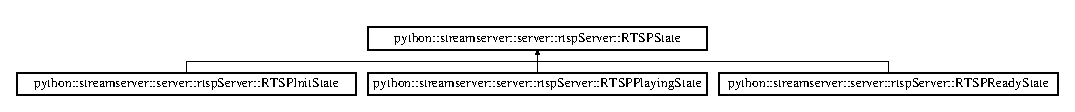
\includegraphics[height=1.054614cm]{classpython_1_1streamserver_1_1server_1_1rtspServer_1_1RTSPState}
\end{center}
\end{figure}
\subsection*{Public Member Functions}
\begin{DoxyCompactItemize}
\item 
\hypertarget{classpython_1_1streamserver_1_1server_1_1rtspServer_1_1RTSPState_ad999577fe54292fe16e2dc4df2ec0146}{
def {\bfseries changeState}}
\label{classpython_1_1streamserver_1_1server_1_1rtspServer_1_1RTSPState_ad999577fe54292fe16e2dc4df2ec0146}

\item 
def \hyperlink{classpython_1_1streamserver_1_1server_1_1rtspServer_1_1RTSPState_a945c1ab744e22499551d8cc5aafa687f}{parseRequest}
\item 
\hypertarget{classpython_1_1streamserver_1_1server_1_1rtspServer_1_1RTSPState_a327a539de88366b5d3833db65f92a333}{
def {\bfseries parseMethodName}}
\label{classpython_1_1streamserver_1_1server_1_1rtspServer_1_1RTSPState_a327a539de88366b5d3833db65f92a333}

\item 
\hypertarget{classpython_1_1streamserver_1_1server_1_1rtspServer_1_1RTSPState_a7093a9574aaf5cbcfaa572feaec456cc}{
def {\bfseries handleOPTIONS}}
\label{classpython_1_1streamserver_1_1server_1_1rtspServer_1_1RTSPState_a7093a9574aaf5cbcfaa572feaec456cc}

\item 
\hypertarget{classpython_1_1streamserver_1_1server_1_1rtspServer_1_1RTSPState_a3138e2a7d2f6b8c28e38f303ce6b1ef9}{
def {\bfseries handleDESCRIBE}}
\label{classpython_1_1streamserver_1_1server_1_1rtspServer_1_1RTSPState_a3138e2a7d2f6b8c28e38f303ce6b1ef9}

\item 
\hypertarget{classpython_1_1streamserver_1_1server_1_1rtspServer_1_1RTSPState_a2b8af08f8d19bad290ad4430ab7c53f9}{
def {\bfseries handleSETUP}}
\label{classpython_1_1streamserver_1_1server_1_1rtspServer_1_1RTSPState_a2b8af08f8d19bad290ad4430ab7c53f9}

\item 
\hypertarget{classpython_1_1streamserver_1_1server_1_1rtspServer_1_1RTSPState_a203d619937ec1d6ea99644d177622707}{
def {\bfseries handlePLAY}}
\label{classpython_1_1streamserver_1_1server_1_1rtspServer_1_1RTSPState_a203d619937ec1d6ea99644d177622707}

\item 
\hypertarget{classpython_1_1streamserver_1_1server_1_1rtspServer_1_1RTSPState_a5104a8a6e63ea8624a5cc52dda357be5}{
def {\bfseries handleTEARDOWN}}
\label{classpython_1_1streamserver_1_1server_1_1rtspServer_1_1RTSPState_a5104a8a6e63ea8624a5cc52dda357be5}

\end{DoxyCompactItemize}


\subsection{Member Function Documentation}
\hypertarget{classpython_1_1streamserver_1_1server_1_1rtspServer_1_1RTSPState_a945c1ab744e22499551d8cc5aafa687f}{
\index{python::streamserver::server::rtspServer::RTSPState@{python::streamserver::server::rtspServer::RTSPState}!parseRequest@{parseRequest}}
\index{parseRequest@{parseRequest}!python::streamserver::server::rtspServer::RTSPState@{python::streamserver::server::rtspServer::RTSPState}}
\subsubsection[{parseRequest}]{\setlength{\rightskip}{0pt plus 5cm}def python::streamserver::server::rtspServer::RTSPState::parseRequest (
\begin{DoxyParamCaption}
\item[{}]{ self, }
\item[{}]{ proto, }
\item[{}]{ lines}
\end{DoxyParamCaption}
)}}
\label{classpython_1_1streamserver_1_1server_1_1rtspServer_1_1RTSPState_a945c1ab744e22499551d8cc5aafa687f}
\begin{DoxyVerb}parse the request lines send from the client\end{DoxyVerb}
 

The documentation for this class was generated from the following file:\begin{DoxyCompactItemize}
\item 
/home/yy/programme/python/streamserver/server/\hyperlink{rtspServer_8py}{rtspServer.py}\end{DoxyCompactItemize}

\hypertarget{classpython_1_1streamserver_1_1server_1_1source_1_1SDPState}{
\section{python::streamserver::server::source::SDPState Class Reference}
\label{classpython_1_1streamserver_1_1server_1_1source_1_1SDPState}\index{python::streamserver::server::source::SDPState@{python::streamserver::server::source::SDPState}}
}
\subsection*{Public Member Functions}
\begin{DoxyCompactItemize}
\item 
\hypertarget{classpython_1_1streamserver_1_1server_1_1source_1_1SDPState_aa36f19b399b12fb25e297cf885400aad}{
def {\bfseries \_\-\_\-init\_\-\_\-}}
\label{classpython_1_1streamserver_1_1server_1_1source_1_1SDPState_aa36f19b399b12fb25e297cf885400aad}

\item 
\hypertarget{classpython_1_1streamserver_1_1server_1_1source_1_1SDPState_aac848f03d5598ee6ab24598170565baf}{
def {\bfseries parseNalu}}
\label{classpython_1_1streamserver_1_1server_1_1source_1_1SDPState_aac848f03d5598ee6ab24598170565baf}

\end{DoxyCompactItemize}


\subsection{Detailed Description}
\begin{DoxyVerb}source has already got the SDP, so extract frame from the nalu \end{DoxyVerb}
 

The documentation for this class was generated from the following file:\begin{DoxyCompactItemize}
\item 
/home/yy/programme/python/streamserver/server/\hyperlink{source_8py}{source.py}\end{DoxyCompactItemize}

\chapter{File Documentation}
\hypertarget{liveStreamServer_8py}{
\section{/home/yy/programme/python/streamserver/server/liveStreamServer.py File Reference}
\label{liveStreamServer_8py}\index{/home/yy/programme/python/streamserver/server/liveStreamServer.py@{/home/yy/programme/python/streamserver/server/liveStreamServer.py}}
}


accpept live stream  


\subsection*{Classes}
\begin{DoxyCompactItemize}
\item 
class \hyperlink{classpython_1_1streamserver_1_1server_1_1liveStreamServer_1_1LiveProtocol}{python::streamserver::server::liveStreamServer::LiveProtocol}
\item 
class \hyperlink{classpython_1_1streamserver_1_1server_1_1liveStreamServer_1_1LiveServer}{python::streamserver::server::liveStreamServer::LiveServer}
\end{DoxyCompactItemize}
\subsection*{Functions}
\begin{DoxyCompactItemize}
\item 
\hypertarget{namespacepython_1_1streamserver_1_1server_1_1liveStreamServer_a22847c5416ec3151696cd299a5b597dc}{
def {\bfseries python::streamserver::server::liveStreamServer::test}}
\label{namespacepython_1_1streamserver_1_1server_1_1liveStreamServer_a22847c5416ec3151696cd299a5b597dc}

\end{DoxyCompactItemize}


\subsection{Detailed Description}
accpept live stream \begin{DoxyAuthor}{Author}
yy 
\end{DoxyAuthor}
\begin{DoxyVersion}{Version}
0.1 
\end{DoxyVersion}
\begin{DoxyDate}{Date}
2012-\/07-\/10 
\end{DoxyDate}

\hypertarget{parser_8py}{
\section{/home/yy/programme/python/streamserver/server/parser.py File Reference}
\label{parser_8py}\index{/home/yy/programme/python/streamserver/server/parser.py@{/home/yy/programme/python/streamserver/server/parser.py}}
}


extract the SDP and each frame from the nalu  


\subsection*{Classes}
\begin{DoxyCompactItemize}
\item 
class \hyperlink{classpython_1_1streamserver_1_1server_1_1parser_1_1NaluParser}{python::streamserver::server::parser::NaluParser}
\end{DoxyCompactItemize}


\subsection{Detailed Description}
extract the SDP and each frame from the nalu \begin{DoxyAuthor}{Author}
y 
\end{DoxyAuthor}
\begin{DoxyVersion}{Version}
0.1 
\end{DoxyVersion}
\begin{DoxyDate}{Date}
2012-\/07-\/12 
\end{DoxyDate}

\hypertarget{rtspHandler_8py}{
\section{/home/yy/programme/python/streamserver/server/rtspHandler.py File Reference}
\label{rtspHandler_8py}\index{/home/yy/programme/python/streamserver/server/rtspHandler.py@{/home/yy/programme/python/streamserver/server/rtspHandler.py}}
}


the details of handle rtsp request  


\subsection*{Classes}
\begin{DoxyCompactItemize}
\item 
class \hyperlink{classpython_1_1streamserver_1_1server_1_1rtspHandler_1_1RTSPRequestHandler}{python::streamserver::server::rtspHandler::RTSPRequestHandler}
\end{DoxyCompactItemize}


\subsection{Detailed Description}
the details of handle rtsp request \begin{DoxyAuthor}{Author}
yy 
\end{DoxyAuthor}
\begin{DoxyVersion}{Version}
0.1 
\end{DoxyVersion}
\begin{DoxyDate}{Date}
2012-\/07-\/07 
\end{DoxyDate}

\hypertarget{rtspServer_8py}{
\section{/home/yy/programme/python/streamserver/server/rtspServer.py File Reference}
\label{rtspServer_8py}\index{/home/yy/programme/python/streamserver/server/rtspServer.py@{/home/yy/programme/python/streamserver/server/rtspServer.py}}
}


Start rtsp session and setup connection with the player.  


\subsection*{Classes}
\begin{DoxyCompactItemize}
\item 
class \hyperlink{classpython_1_1streamserver_1_1server_1_1rtspServer_1_1RTSPState}{python::streamserver::server::rtspServer::RTSPState}
\item 
class \hyperlink{classpython_1_1streamserver_1_1server_1_1rtspServer_1_1RTSPInitState}{python::streamserver::server::rtspServer::RTSPInitState}
\item 
class \hyperlink{classpython_1_1streamserver_1_1server_1_1rtspServer_1_1RTSPReadyState}{python::streamserver::server::rtspServer::RTSPReadyState}
\item 
class \hyperlink{classpython_1_1streamserver_1_1server_1_1rtspServer_1_1RTSPPlayingState}{python::streamserver::server::rtspServer::RTSPPlayingState}
\item 
class \hyperlink{classpython_1_1streamserver_1_1server_1_1rtspServer_1_1RTSPServerProtocol}{python::streamserver::server::rtspServer::RTSPServerProtocol}
\item 
class \hyperlink{classpython_1_1streamserver_1_1server_1_1rtspServer_1_1RTSPServerFactory}{python::streamserver::server::rtspServer::RTSPServerFactory}
\end{DoxyCompactItemize}
\subsection*{Functions}
\begin{DoxyCompactItemize}
\item 
\hypertarget{namespacepython_1_1streamserver_1_1server_1_1rtspServer_ab5fc9002c965f367e69fbcca906829f1}{
def {\bfseries python::streamserver::server::rtspServer::test}}
\label{namespacepython_1_1streamserver_1_1server_1_1rtspServer_ab5fc9002c965f367e69fbcca906829f1}

\end{DoxyCompactItemize}


\subsection{Detailed Description}
Start rtsp session and setup connection with the player. \begin{DoxyAuthor}{Author}
yy 
\end{DoxyAuthor}
\begin{DoxyVersion}{Version}
0.1 
\end{DoxyVersion}
\begin{DoxyDate}{Date}
2012-\/07-\/05 
\end{DoxyDate}

\hypertarget{source_8py}{
\section{/home/yy/programme/python/streamserver/server/source.py File Reference}
\label{source_8py}\index{/home/yy/programme/python/streamserver/server/source.py@{/home/yy/programme/python/streamserver/server/source.py}}
}


LiveSource and FileSource.  


\subsection*{Classes}
\begin{DoxyCompactItemize}
\item 
class \hyperlink{classpython_1_1streamserver_1_1server_1_1source_1_1NoSDPState}{python::streamserver::server::source::NoSDPState}
\item 
class \hyperlink{classpython_1_1streamserver_1_1server_1_1source_1_1SDPState}{python::streamserver::server::source::SDPState}
\item 
class \hyperlink{classpython_1_1streamserver_1_1server_1_1source_1_1LiveSource}{python::streamserver::server::source::LiveSource}
\end{DoxyCompactItemize}


\subsection{Detailed Description}
LiveSource and FileSource. \begin{DoxyAuthor}{Author}
yy 
\end{DoxyAuthor}
\begin{DoxyVersion}{Version}
0.1 
\end{DoxyVersion}
\begin{DoxyDate}{Date}
2012-\/07-\/11 
\end{DoxyDate}

\printindex
\end{document}
